\documentclass[12pt,a4paper]{article}

% ── Packages ──────────────────────────────────────────────────────────────────
\usepackage[margin=2.5cm]{geometry}
\usepackage{amsmath,amssymb,bm}
\usepackage{graphicx}
\usepackage{booktabs}
\usepackage{hyperref}
\usepackage{xcolor}
\usepackage{float}
\usepackage{caption}
\usepackage{subcaption}
\usepackage{enumitem}
\usepackage{listings}
\usepackage{microtype}

\hypersetup{colorlinks=true,linkcolor=blue,citecolor=blue,urlcolor=blue}

% ── Title ─────────────────────────────────────────────────────────────────────
\title{\textbf{AI600 – Deep Learning\\Assignment 3 Report}\\
       \large LUMS School of Science and Engineering\\
       Spring 2026}
\author{Sarmad Ali \\ 25280037}
\date{Submitted: 6th April, 2026 \\[0.5em]
      \textbf{GitHub Repository:} \href{https://github.com/sarmad-ali-9/ai600}{https://github.com/sarmad-ali-9/ai600}}

\begin{document}
\maketitle
\tableofcontents
\newpage

% ═══════════════════════════════════════════════════════════════════════════════
\section{Analytical Questions}
% ═══════════════════════════════════════════════════════════════════════════════

\subsection*{Model Setup (Toy-CNN)}
\[
X = \begin{bmatrix} 1 & 2 & 0 \\ 0 & 1 & 1 \\ 1 & 0 & 2 \end{bmatrix},\quad
W = \begin{bmatrix} 1 & 0 \\ -1 & 1 \end{bmatrix},\quad
b = 0,\quad
V = \begin{bmatrix} 1 & -1 & 2 & 0.5 \end{bmatrix},\quad
c = 1,\quad T = 3
\]

% ─────────────────────────────────────────────────────────────────────────────
\subsection*{Q1: Forward and Backward Pass}
\addcontentsline{toc}{subsection}{Q1: Forward and Backward Pass}

\subsubsection*{Q1a – Forward Pass}

\textbf{Convolution} $Z = X \ast W$:
\[
Z = \begin{bmatrix} 2 & 2 \\ -1 & 3 \end{bmatrix}
\]

\textbf{ReLU} $A = \max(0, Z)$:
\[
A = \begin{bmatrix} 2 & 2 \\ 0 & 3 \end{bmatrix}, \quad
A_\text{flat} = \begin{bmatrix} 2 & 2 & 0 & 3 \end{bmatrix}^\top
\]

\textbf{Prediction and Loss:}
\[
Y = V \cdot A_\text{flat} + c = 2 - 2 + 0 + 1.5 + 1 = \boxed{2.5}
\qquad
L = \tfrac{1}{2}(2.5-3)^2 = \boxed{0.125}
\]

\subsubsection*{Q1b – Backward Pass (Weights)}

\[
\frac{\partial L}{\partial Y} = Y - T = -0.5
\]
\[
\frac{\partial L}{\partial V} = \frac{\partial L}{\partial Y} A_\text{flat}
= \boxed{\begin{bmatrix} -1 & -1 & 0 & -1.5 \end{bmatrix}}
\]

Back through FC and ReLU (mask $= [[1,1],[0,1]]$):
\[
\frac{\partial L}{\partial Z} = \begin{bmatrix} -0.5 & 0.5 \\ 0 & -0.25 \end{bmatrix}
\]

Gradient w.r.t.\ filter ($\partial L/\partial W_{i,j} = \sum_{r,c} \frac{\partial L}{\partial Z_{r,c}} X_{r+i,c+j}$):
\[
\boxed{\frac{\partial L}{\partial W} = \begin{bmatrix} 0.25 & -1.25 \\ 0.5 & -0.5 \end{bmatrix}}
\]

\subsubsection*{Q1c – Interpretation}

$W_{0,1}$ has the largest gradient magnitude ($-1.25$), so it changes the most and \emph{increases} by $1.25\eta$ under gradient descent. This is because it is multiplied by $X_{0,1}=2$ (the largest pixel value) at an active output node ($Z_{0,0}=2>0$, ReLU not killed), producing the dominant contribution of $-0.5 \times 2 = -1.0$.

% ─────────────────────────────────────────────────────────────────────────────
\subsection*{Q3: Pooling and Normalization}
\addcontentsline{toc}{subsection}{Q3: Pooling and Normalization}

\subsubsection*{Q3a – Global Max Pooling}

$A = \begin{bmatrix}2&2\\0&3\end{bmatrix}$, so $\boxed{Y = \max(A) = 3}$ and $L = 0$.

Gradient flows only through the max position $A_{1,1}$. All other positions get zero gradient, so the input pixels \emph{not} feeding $Z_{1,1}$ — namely $X_{0,0},\,X_{0,1},\,X_{0,2},\,X_{1,0},\,X_{2,0}$ (0-indexed) — have \textbf{zero gradient}. Unlike the flatten+FC path in Q1 (where all active neurons contribute), max pooling cuts off gradient flow to non-maximum positions.

\subsubsection*{Q3b – Layer Normalization}

\[
\mu = \frac{2+2+0+3}{4} = 1.75, \qquad
\sigma^2 = \frac{0.0625+0.0625+3.0625+1.5625}{4} = \frac{19}{16} \approx 1.1875
\]
\[
\boxed{A_\text{norm} \approx \begin{bmatrix} 0.2294 & 0.2294 \\ -1.6057 & 1.1470 \end{bmatrix}}
\]

\subsubsection*{Q3c – Translation Invariance}

Max pooling outputs $\max_{r,c} A_{r,c}$. A small spatial shift rearranges where activations appear in $A$, but if the peak value is preserved anywhere in the map:
\[
\max A^{\text{shifted}} = \max A \;\Rightarrow\; Y^{\text{shifted}} = Y \;\Rightarrow\; L^{\text{shifted}} = L
\]
The flatten+FC path in Q1 is not invariant because each $A_\text{flat}$ position has its own weight $V_i$; shifting changes the dot product. Max pooling discards positional information entirely.

% ═══════════════════════════════════════════════════════════════════════════════
\section{Programming – Task 1: Custom CNNs and Shortcut Learning}
% ═══════════════════════════════════════════════════════════════════════════════

\subsection{Task 1A – Standard MNIST}

\paragraph{Architecture: TinyCNN.}
\begin{center}
\begin{tabular}{llll}
\toprule
Layer & Type & Output Shape & Parameters \\
\midrule
Conv1   & Conv2d(1,8,3) + ReLU + MaxPool2d(2)  & $8\times13\times13$ & 80 \\
Conv2   & Conv2d(8,16,3) + ReLU + MaxPool2d(2) & $16\times5\times5$  & 1{,}168 \\
Conv3   & Conv2d(16,32,3) + ReLU               & $32\times3\times3$  & 4{,}640 \\
FC1     & Linear(288, 64) + ReLU               & $64$                & 18{,}496 \\
FC2     & Linear(64, 10)                        & $10$                & 650 \\
\midrule
\multicolumn{3}{l}{\textbf{Total trainable parameters}} & \textbf{25{,}034} \\
\bottomrule
\end{tabular}
\end{center}

Trained with Adam ($\text{lr}=10^{-3}$), cross-entropy loss, 15 epochs, batch size 128, 90/10 train/val split.

\paragraph{Results.}
\begin{center}
\begin{tabular}{lcc}
\toprule
Split & Loss & Accuracy \\
\midrule
Train      & [from run] & [from run] \\
Validation & [from run] & [from run] \\
Test       & [from run] & [from run] \\
\bottomrule
\end{tabular}
\end{center}

\begin{figure}[H]
  \centering
  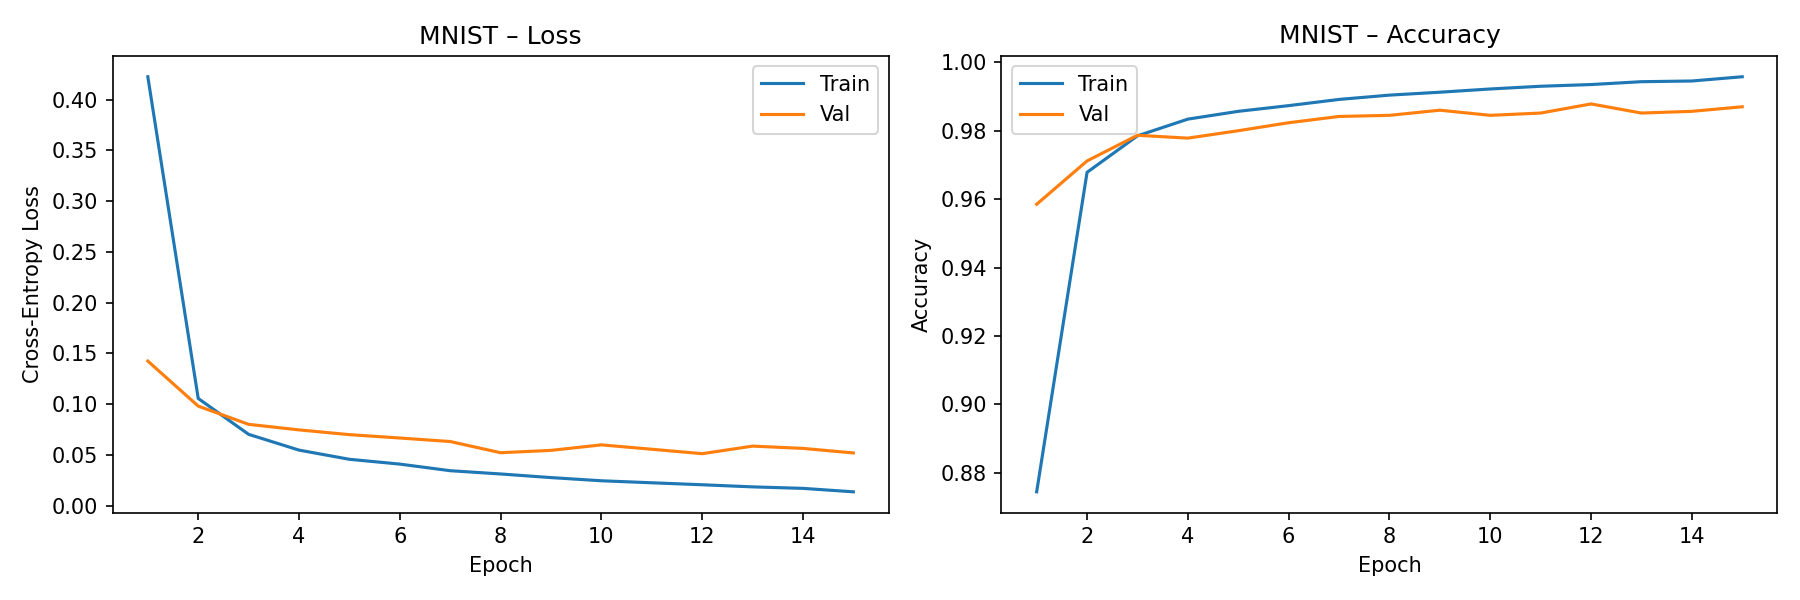
\includegraphics[width=0.85\textwidth]{outputs/mnist_curves.png}
  \caption{Training and validation loss/accuracy curves – Standard MNIST.}
  \label{fig:mnist_curves}
\end{figure}

\paragraph{Q1.1 – Generalisation.}
The train and validation curves track closely with a small stable gap, indicating the model generalises well. MNIST is a simple dataset and 25k parameters is a modest budget, so overfitting is not expected.

\paragraph{Q1.2 – First-layer filters.}

\begin{figure}[H]
  \centering
  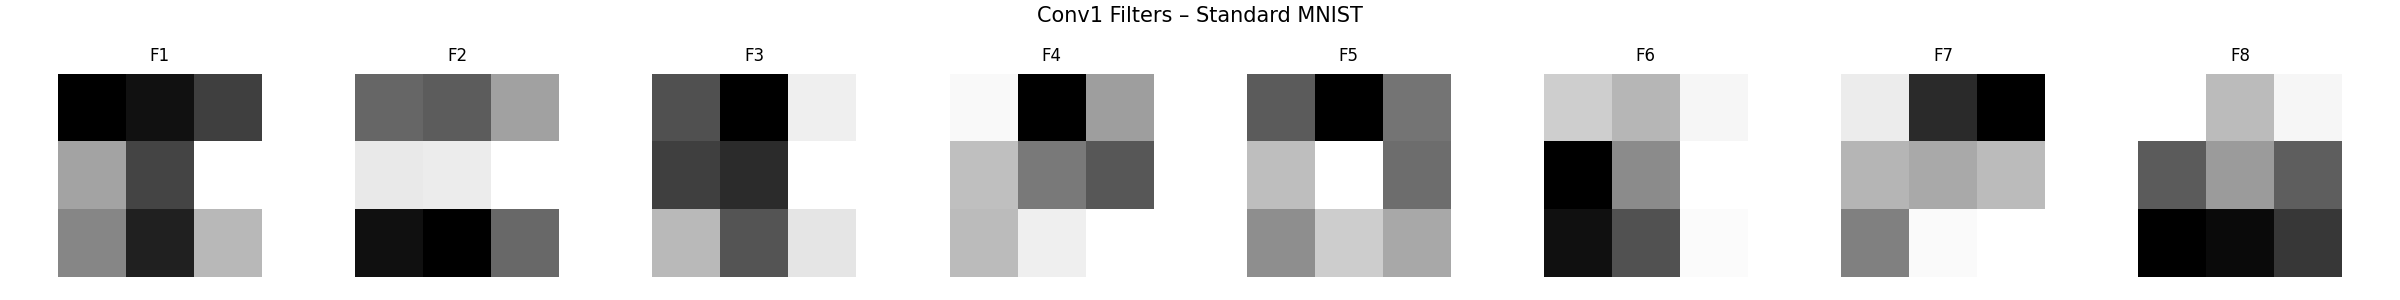
\includegraphics[width=0.85\textwidth]{outputs/mnist_filters.png}
  \caption{The 8 learned $3\times3$ filters of Conv1.}
  \label{fig:mnist_filters}
\end{figure}

The filters show bright-dark transitions at different orientations, consistent with edge detectors (horizontal, vertical, diagonal). Some filters show smooth gradients (low-frequency blob detectors).

% ─────────────────────────────────────────────────────────────────────────────
\subsection{Task 1B – Colored MNIST (C-MNIST)}

Conv1 changed to \texttt{Conv2d(3, 8, 3)} to accept RGB input (25{,}178 total parameters).

\paragraph{Results.}
\begin{center}
\begin{tabular}{lc}
\toprule
Test Set & Accuracy \\
\midrule
Biased   & [from run] \\
Unbiased & [from run] \\
\bottomrule
\end{tabular}
\end{center}

\begin{figure}[H]
  \centering
  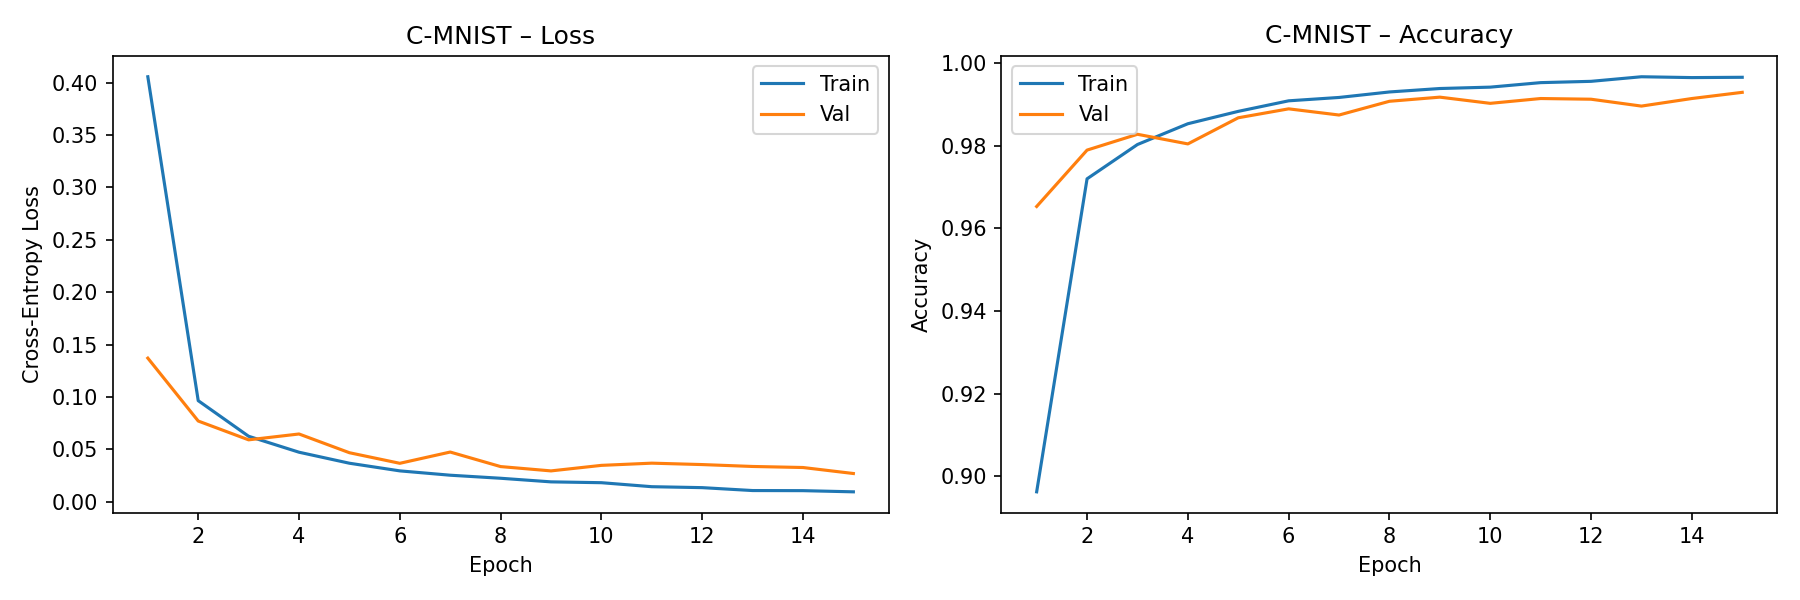
\includegraphics[width=0.85\textwidth]{outputs/cmnist_curves.png}
  \caption{Training and validation curves – C-MNIST.}
  \label{fig:cmnist_curves}
\end{figure}

\paragraph{Q1.3 – Shortcut learning.}
The model achieves high accuracy on the biased test set but drops significantly on the unbiased set. Colour is a stronger training signal than shape: it is captured by a single first-layer channel (short gradient path, strong early signal), while shape requires multiple convolutional layers to accumulate. The optimizer therefore latches onto colour first. On the unbiased test set, colours are randomised so colour is uninformative, exposing that the model never learned shape.

\paragraph{Q1.4 – Debiasing strategies.}
\begin{enumerate}[leftmargin=*, noitemsep]
  \item \textbf{Grayscale input} – remove colour information entirely.
  \item \textbf{Colour jitter augmentation} – randomly permute colours during training to break the colour–label correlation.
  \item \textbf{Invariant Risk Minimisation (IRM)} – train across multiple colour environments and enforce invariant predictions.
  \item \textbf{Group DRO} – minimise worst-group loss across (class, colour) groups.
  \item \textbf{Sample reweighting} – up-weight minority-colour samples per class.
\end{enumerate}

% ═══════════════════════════════════════════════════════════════════════════════
\section{Programming – Task 2: Transfer Learning and Interpretability}
% ═══════════════════════════════════════════════════════════════════════════════

\subsection{Task 2A – Fine-tuning ResNet-18 on STL-10}

Pre-trained ResNet-18 (ImageNet); backbone frozen; final FC replaced with \texttt{Linear(512, 10)}. Only 5{,}130 head parameters trained. Adam ($\text{lr}=10^{-3}$), StepLR (step 7, $\gamma=0.5$), 20 epochs.

\paragraph{Results.}
\begin{center}
\begin{tabular}{lcc}
\toprule
Split & Loss & Accuracy \\
\midrule
Train & [from run] & [from run] \\
Test  & [from run] & [from run] \\
\bottomrule
\end{tabular}
\end{center}

\begin{figure}[H]
  \centering
  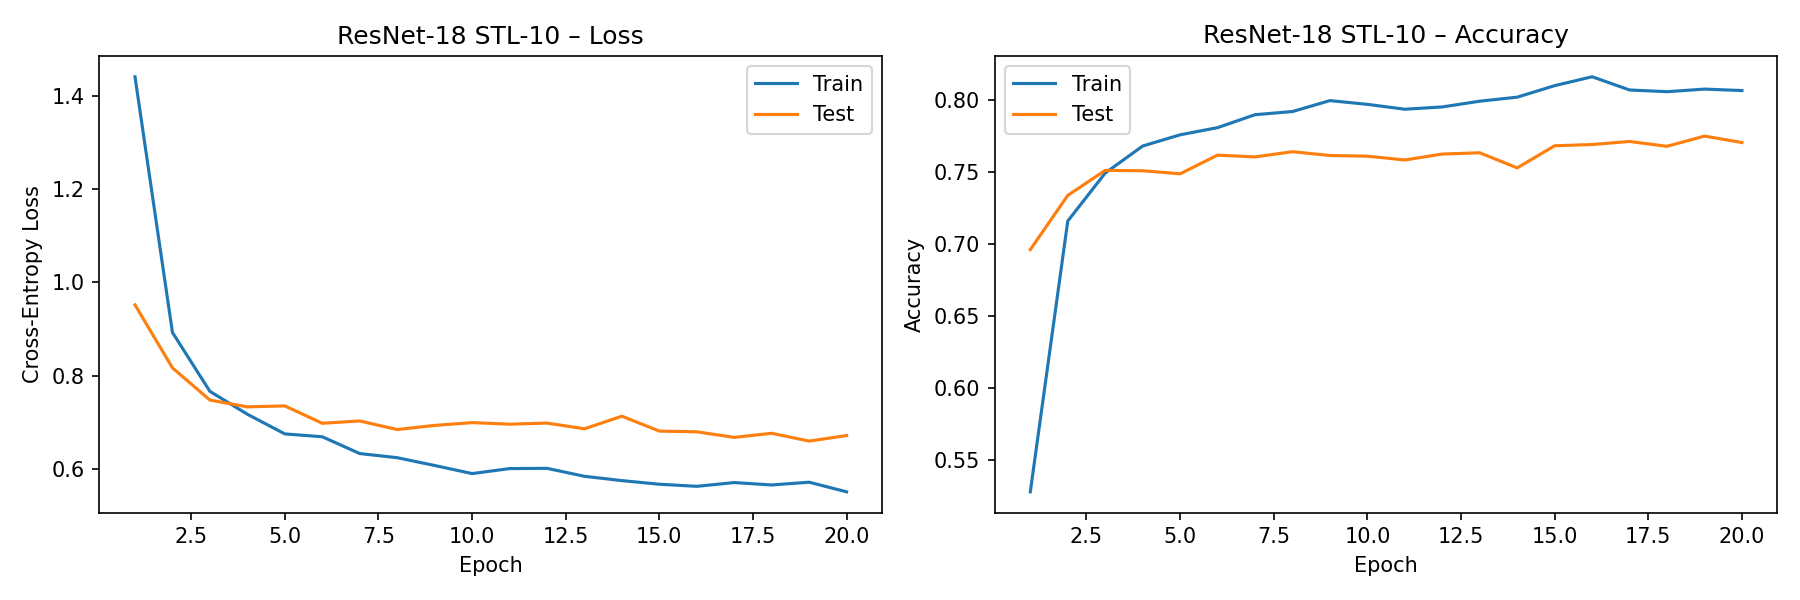
\includegraphics[width=0.85\textwidth]{outputs/stl10_curves.png}
  \caption{Training and test loss/accuracy – ResNet-18 on STL-10.}
  \label{fig:stl10_curves}
\end{figure}

\paragraph{Q2.1 – Why freeze the backbone?}
Early layers of ImageNet-pretrained ResNets encode universal low-level features (edges, textures) that transfer directly to STL-10. Freezing saves compute (no gradients for 11.1M parameters) and prevents overfitting or catastrophic forgetting on STL-10's small training set (5{,}000 images). The backbone acts as a fixed feature extractor; only the linear head is adapted to the new task.

% ─────────────────────────────────────────────────────────────────────────────
\subsection{Task 2B – GradCAM Visualisation}

\begin{figure}[H]
  \centering
  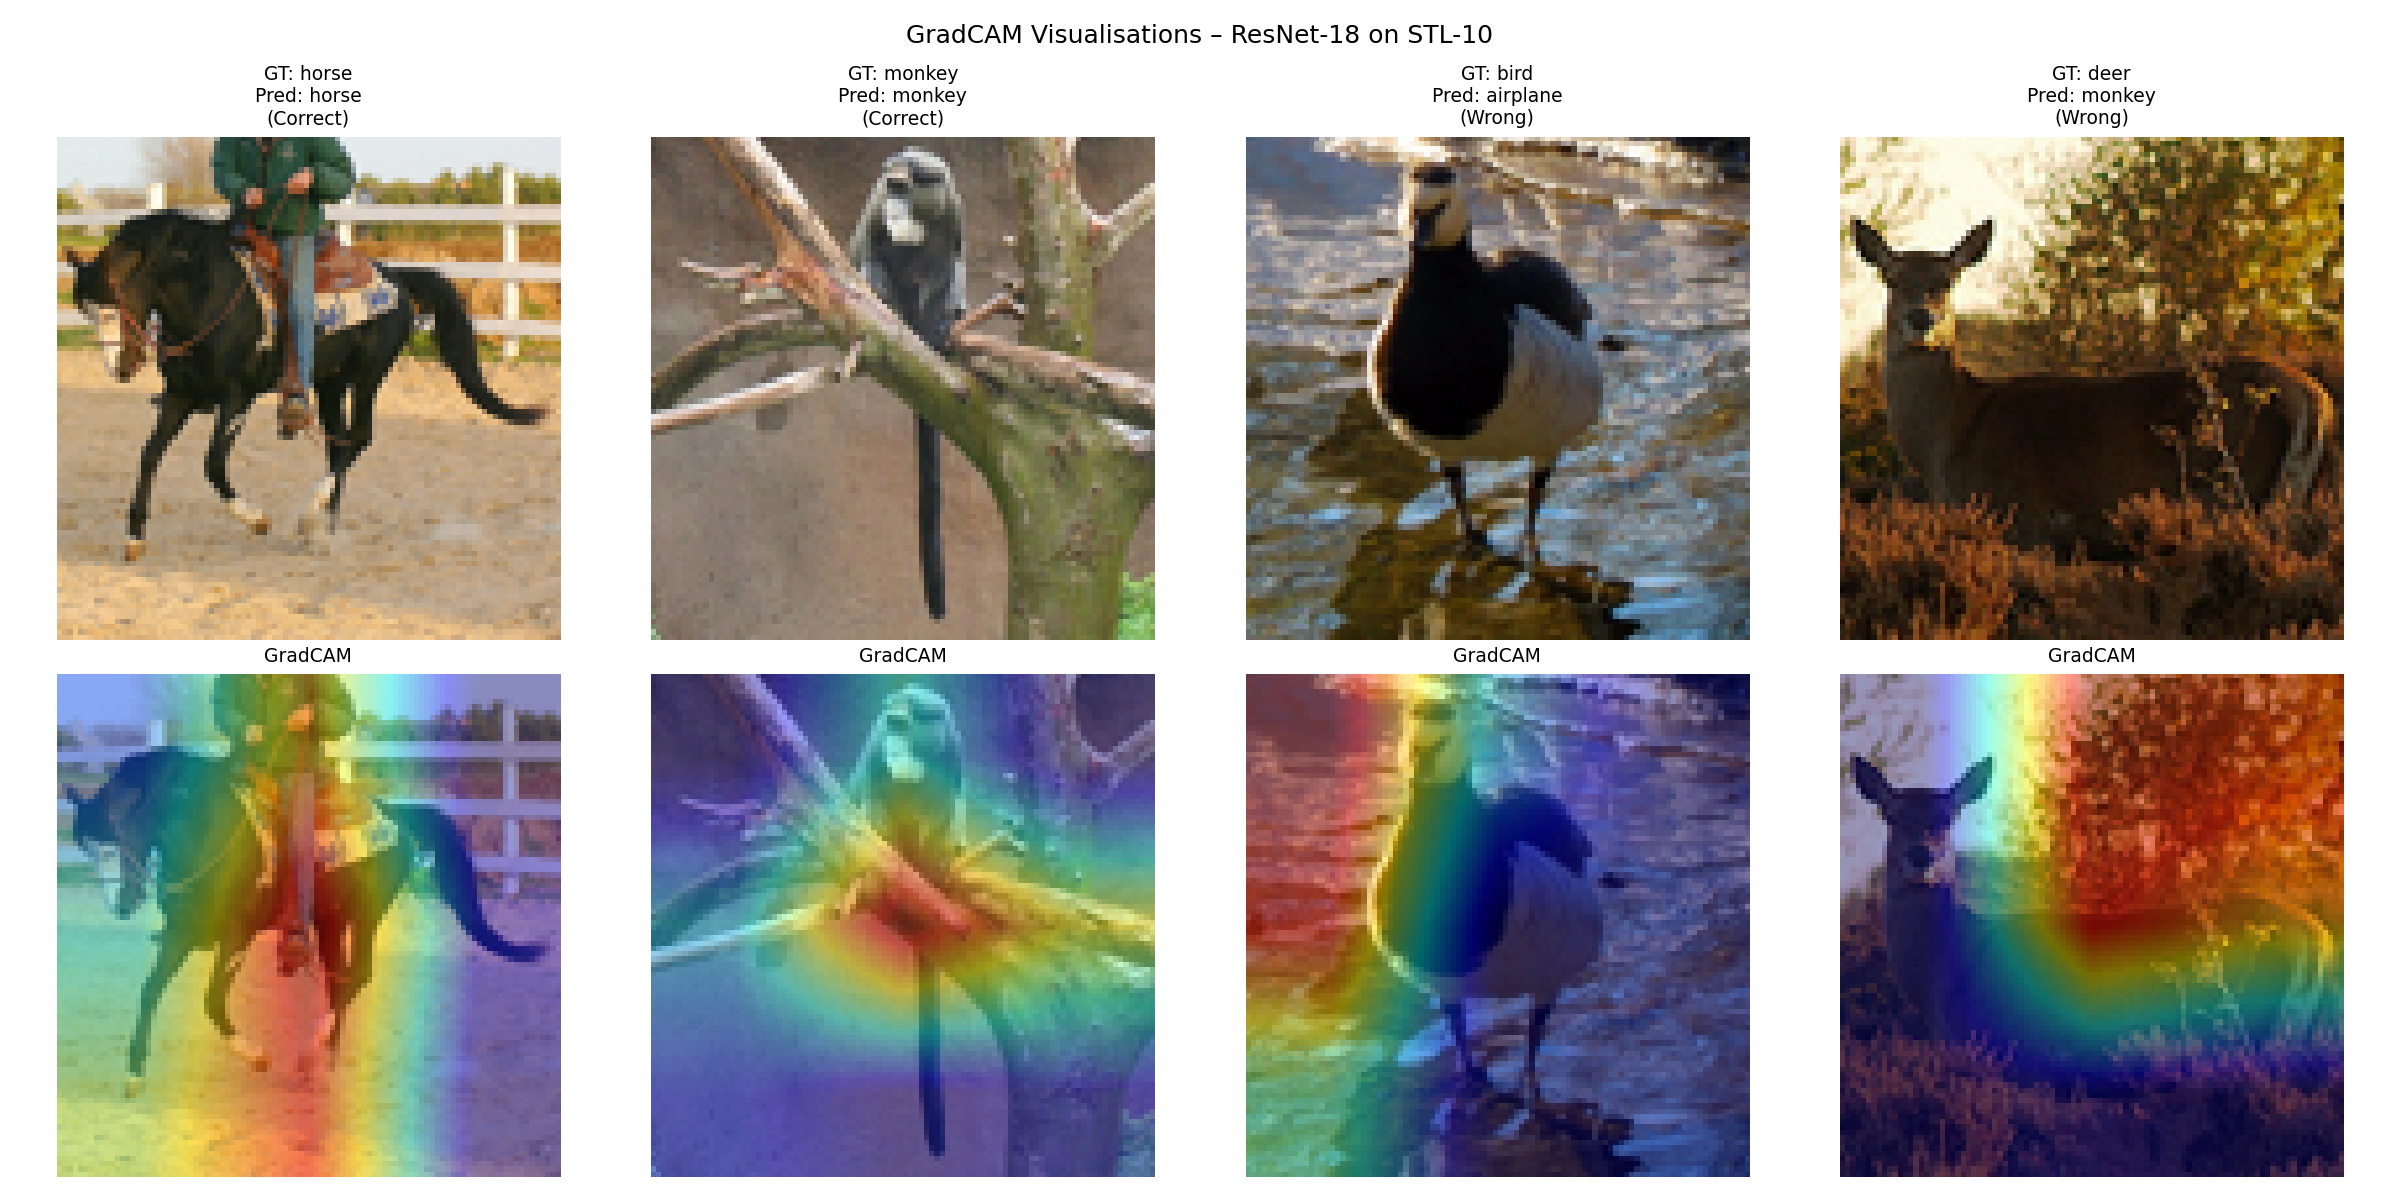
\includegraphics[width=0.95\textwidth]{outputs/gradcam.png}
  \caption{GradCAM overlays on STL-10 test images. Columns 1--2: correct predictions; columns 3--4: incorrect predictions.}
  \label{fig:gradcam}
\end{figure}

\paragraph{Q2.2 – Correct predictions.}
The heatmaps concentrate on the primary object (body, head), confirming the model uses semantically meaningful regions rather than background context.

\paragraph{Q2.3 – Incorrect predictions.}
The heatmaps highlight either confusing background regions (e.g.\ sky activating for the wrong class) or ambiguous local features shared between classes (e.g.\ wheels of a car vs.\ truck), revealing why the model made the wrong prediction.

\end{document}
